%---------- COURSE INFORMATION ------------------------
\newcommand{\course}{ITE 369-01}
\newcommand{\coursetitle}{USABLE PRIVACY AND SECURITY}
\newcommand{\courseloc}{Keller 234}
\newcommand{\coursetime}{Monday/Wednesday 3 - 4:15 p.m.}
\newcommand{\coursedesc}{This course investigates privacy and security from a user-centered point of view. How do people think about privacy and security? How do they interact with current applications and solutions? What should be considered in designing user-friendly security systems? This course introduces students to a variety of usability and user interface issues related to privacy and security and examines potential designs and solutions.}

\newcommand{\coursesec}{01}
\newcommand{\coursecredithours}{3}
\newcommand{\courseprereq}{ITE 249.}
\newcommand{\coursedelmethod}{Hybrid}

\newcommand{\courseobjectives}{
	\item Explain the usability and security principles of interactive systems and how to address/solve problems in both areas.
	\item Evaluate usability aspects associated with secure mechanisms and protections, such as: encryption, access control, and authentication.
	\item Explain security problems associated primarily with humans, such as: phishing and other social engineering attacks, warnings and end-user security education.
}

\newcommand{\coursetopics}{\item Usability of Interactive Systems
	\item User Foundations
	\item Privacy 
	\item Privacy notifications and controls
	\item Encryption
	\item End user access control
	\item Authentication
	\item Warnings
	\item Phishing and social engineering
	\item End user security knowledge and tools
	\item Tracking 
	\item Social behavioral privacy
	\item Administrators and Expert tools
	\item Design Principles and process
	\item Security and Privacy processes
	\item User studies of security and privacy
}
\newcommand{\coursegrades}{Subject Exams (4 exams)\dotfillsmall 70\% \\
Comprehensive Final Exam\dotfillsmall 30\%}
\newcommand{\coursetext}{ & Course text and readings will be selected from current research papers and e-book chapters. I will provide a download or internet link to these reading sources via Canvas.
%	\adjustbox{valign=c}{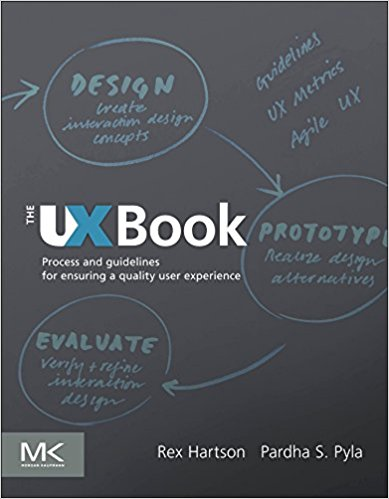
\includegraphics[width=1in]{img/cis489}} & \hangindent .4in \textbf{Textbook:} Hartson, R., Pyla, P., (2012)., he UX Book: Process and Guidelines for Ensuring a Quality User Experience (1st edition). Morgan Kaufmann. ISBN-10: 0123852412, ISBN-13: 978-0123852410. \\
	%& \hangindent .4in Simulation Software: SAM 365 \& 2016 Assessments, Trainings, and Projects with MindTap Reader.
}